\documentclass[border=0mm,tikz]{standalone}
\usepackage{times}
\usetikzlibrary{shapes}
\usetikzlibrary{calc}

% TikZ styles
\tikzstyle{block} = [draw, rectangle, fill=gray!5, rounded corners,
                     text centered, minimum height=1cm]
\tikzstyle{trunk}  = [block, text width=55mm, minimum width=60mm]
\tikzstyle{branch} = [block, text width=32.5mm, minimum width=35mm]
\tikzstyle{split} = [draw, diamond, fill=gray!5, minimum size=2.5cm]
\newcommand{\PDD}{\mathrm{PDD}}
\newcommand{\SMB}{\mathrm{SMB}}

% begin document
\begin{document}
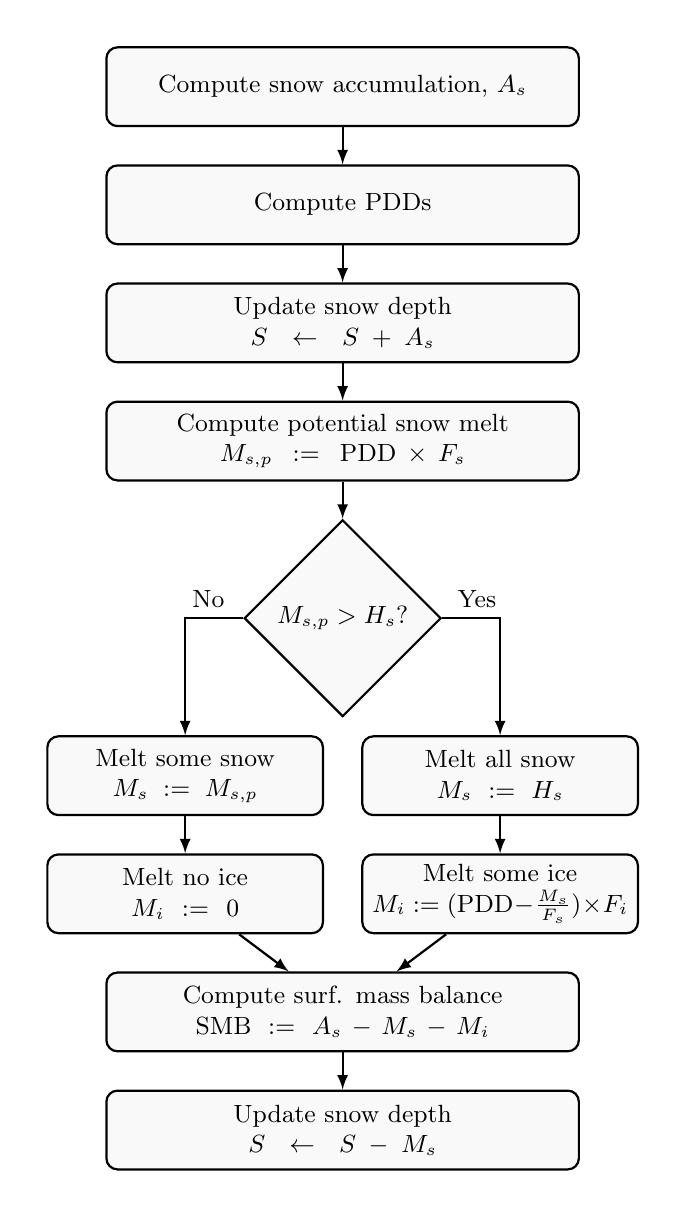
\begin{tikzpicture}[thick, font=\small, >=latex]

% background
\fill[white] (0,0) rectangle +(8.0,14.75);
%\draw[help lines, lightgray] (0,0) grid (8,14);

% add nodes
\path     (4, 14) node [trunk] (acc) {Compute snow accumulation, $A_s$}
  -- ++(0, -1.5) node [trunk] (pdd) {Compute PDDs}
  -- ++(0, -1.5) node [trunk]  (s1) {Update snow depth \\
                                      $S \gets S + A_s$}
  -- ++(0, -1.5) node [trunk] (msp) {Compute potential snow melt \\
                                      $M_{s,p} := \PDD \times F_{s}$}
  -- ++(0, -2.25) node [split] (split) {$M_{s,p} > H_s?$};

\path ($(split)+(-2,-2)$) node [branch] (no)  {Melt some snow \\
                                               $M_s := M_{s,p}$}
  -- ++(0, -1.5) node [branch] (nomi) {Melt no ice \\
                                      $M_i := 0$};


\path ($(split)+(+2,-2)$) node [branch] (yes) {Melt all snow \\
                                               $M_s := H_s$}
  -- ++(0, -1.5) node [branch] (yesmi) {Melt some ice \\
                                        $M_i := (\PDD - \frac{M_s}{F_s}) \times F_i$};

\path ($(split)+(0,-5)$) node [trunk](smb) {Compute surf. mass balance \\
                                      $\SMB := A_s - M_s - M_i$}
  -- ++(0, -1.5) node [trunk]  (s2) {Update snow depth \\
                                      $S \gets S - M_s$};

% add connections
\draw[->] (acc) -- (pdd);
\draw[->] (pdd) -- (s1);
\draw[->] (s1) -- (msp);
\draw[->] (msp) -- (split);
\draw[->] (split) -| (no) node [pos=0.3, above] {No};
\draw[->] (no) -- (nomi);
\draw[->] (nomi) -- (smb);
\draw[->] (split) -| (yes) node [pos=0.3, above] {Yes};
\draw[->] (yes) -- (yesmi);
\draw[->] (yesmi) -- (smb);
\draw[->] (smb) -- (s2);

\end{tikzpicture}
\end{document}
